%
% Barren Planet - User Manual
% Main document source
%
% Copyright (C) Damian Gareth Walker 2022
% Manual Sections: Repair and Construction
%
% Structure:
% Resources
% Repairing Units
% Building New Units
% Build Restrictions
%

% Chapter Title
\chapter{Repair and Construction}

% Introductory
\noindent
The first battle in {\it First Landing} is a simple one where the units initially deployed are all you get, during the battle. But in subsequent battles, {\bf \it Barren Planet} introduces some interesting abilities: the abilities to repair and build units on the battlefield.

% Resources
\section{Resources}

% Introductory
\noindent
Repair and building require {\it resources}. At the start of each battle, each side is allocated a certain amount of resources for building and repair. In some battles this is all you get, and you will have to carefully eke out these resources to last until the battle is won.

% Illustrating resources
\begin{figure}[h]
  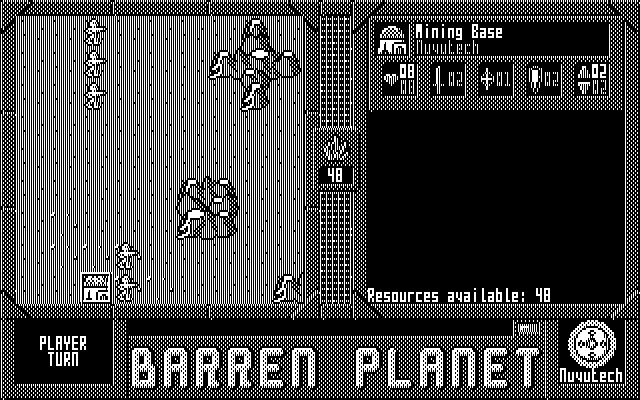
\includegraphics[width=\textwidth]{starting-resources}
  \caption{Now is the time to start paying attention to the messages
    about resources, and the display in the centre of the screen.}
\end{figure}

% Gathering Resources
In other battles the resources can be gathered turn by turn. Resources are generated by the {\it Crystal Nodes} when occupied by a {\it Mining Base}. Each Mining Base occupying a Crystal Node gains 2 resource points per turn for its side. If the opponent destroys a Mining Base, the income from that Crystal Node is cut off for the rest of the battle. So it is a valid tactic to target the enemy's Mining Bases early, in order to starve them of resources for future repair and construction.

% Display
Your current resources are shown in a small pop-out window in the centre of the screen, nestled between the map window and the report message window: look for the crystal node symbol. The report messages will also update you on available resources at the start of your turn, and every time you spend resources in building and construction.

% Repair
\section{Repairing Damaged Units}

% Role of the Mining Base
\noindent
As well as gathering resources, the {\it Mining Base} can also be used to repair damaged units. If there are resources enough, a Mining Base can repair up to two adjacent friendly units each turn. The repair cost of a unit is half its build cost, as listed in the Appendix.

% Illustrating Unit Selection
\begin{figure}[h]
  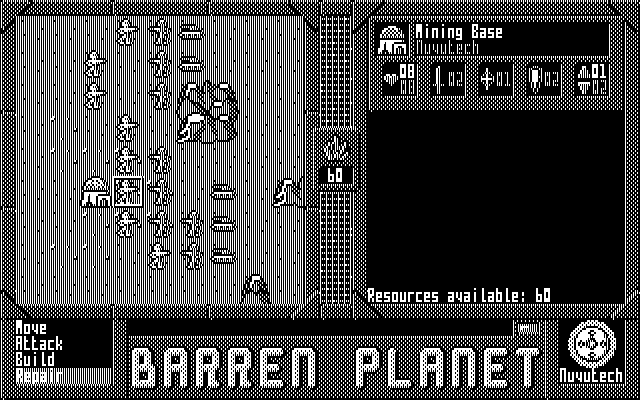
\includegraphics[width=\textwidth]{unit-repair}
  \caption{Repairing a damaged unit.}
\end{figure}

% Retreating Damaged Units
When repair comes into play, damaged units are no longer regarded as lame ducks to be used as sacrifices or decoys. Now there is a purpose to retreat: you can draw damaged units back to your Mining Bases where they can be repaired and sent back into battle at full strength.

% Getting this capability
The quickest way to gain access to the repair ability is to win the first battle of {\it First Landing}. So if you played that battle and lost, start a new game and try again. And again if necessary, until you come out victorious. Your second battle will then begin with a Mining Base deployed. Now you can send your units into battle with renewed confidence, despite the fact that you are outnumbered.

% Taking Damage
Continue the fight until one of your Combat Droids has its hit points reduced by at least half. Now it is time to withdraw: while the other Combat Droids continue the fight, move the damaged Combat Droid back each turn till it is adjacent to the Mining Base. Once that's done, you are ready to repair it.

% Controls
With the Combat Droid adjacent, move the cursor to the Mining Base and tap {\it fire} to select it. Move the cursor back to the damaged Combat Droid and tap {\it fire} again. This won't select the Combat Droid as you'd expect. If your current unit is a Mining Base, and you point at an adjacent friendly unit, the default menu option becomes {\it Repair} instead. You should see a spanner briefly appear over the Combat Droid, and then a report message will confirm that the Combat Droid has been repaired. Your resources will be reduced by the appropriate amount.

% Selecting the Repaired Unit
To select the Combat Droid to verify it is at full strength, you will need to hold {\it fire} and choose the {\it Select} option to select it. If it has movement points remaining, it can immediately move back towards the battle front.

% Tactics
It is important to keep an eye on your units' hit points and not allow them to be needlessly destroyed. This is especially true in this second battle, where you are outnumbered by the enemy. If you don't keep your units in good repair then you will be easily overcome. It might be a good idea in this scenario to keep your Combat Droids close to the Mining Base and let the enemy come to you. That way your units will not have a long journey when they need to retreat for repair.

% Building New Units
\section{Building New Units}

% Getting There
\noindent
Part way through the campaign, your Mining Bases will gain the ability to build new units during the battle. Then you'll not be limited to the units that are initially deployed, but you can add your to your forces other units that you find useful. The rest of this section assumes you have arrived at such a battle.

% Illustrating Unit Selection
\begin{figure}[h]
  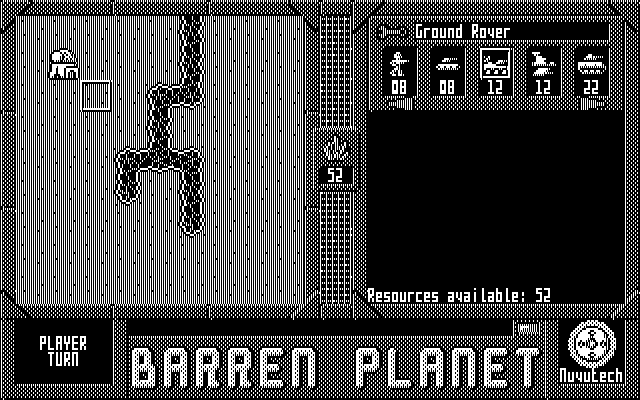
\includegraphics[width=\textwidth]{unit-build}
  \caption{The Unit Selection presented when you Build.}
\end{figure}

% Controls
To build a new unit, move the cursor to a Mining Base and tap {\it fire} to select it. Then move the cursor to an adjacent empty square and tap {\it fire} again to choose the {\it Build} option from the menu. When a Mining Base is selected, the default option when pointing at an adjacent empty square becomes {\it Build}, rather than {\it Move} as it would be for other units.

% Unit Selection
The stats panel will change to a format you've not seen before. This is the {\it Unit Selection}. The upper text box shows the unit type selected, while all the unit types are shown in the icon boxes beneath. Beneath each unit icon is the resource cost to build it. There is a cursor in one of the boxes, and as you move that cursor with the $\leftarrow$ and $\rightarrow$ controls, the upper text box will change to the name of the highlighted unit. If there are move than five units that you can build, you can scroll past the fifth unit to see more of them.

% Build Menu
When you have highlighted the unit you want to build, tap {\it fire} to choose the default {\it Build} option from the Build Menu. If you have changed your mind about building, you can instead hold {\it fire} and choose the {\it Cancel} option instead.

% The New Arrival
Once you have selected a unit and chosen {\it Build}, a spanner symbol will appear briefly on the map, and then the unit will be built. The new unit will start off with no movement points, so it will not be able to move this turn, nor will it be able to return fire if it is attacked before its next turn. So take care to protect your new unit unless it is itself exceptionally robust.

% Restrictions on Building
\section{Restrictions on Building}

% Unit capabilities
\noindent
Mining Bases are able to build and repair any of the mobile units: Combat Droids, Hoverbugs, Ground Rovers, Air Fighers, Laser Tanks and Laser Cannon. They cannot build or repair  Gun Platforms or other Mining Bases. So you must take care to defend your static units.

% Scenario capabilities
In some early battles, the Mining Bases lack the facility to build new units, and in other battles the Mining Bases may be limited on which other units they can build. But they can always repair any of the mobile units.
